\documentclass[11pt]{article}
%Gummi|065|=)
\usepackage{listings}
\lstset{language=C}
\usepackage[utf8]{inputenc}
\usepackage[T1]{fontenc}
\usepackage{epstopdf}
\usepackage{lmodern}
\usepackage{amsmath}
\usepackage{geometry}
\usepackage{color}
\usepackage{xcolor}
\usepackage{listings}
\usepackage{graphicx}

\usepackage{caption}
\geometry {a4paper, top=25mm, left=25mm, right=25mm, bottom=25mm}
\DeclareCaptionFont{white}{\color{white}}
\DeclareCaptionFormat{listing}{\colorbox{gray}{\parbox{\textwidth}{#1#2#3}}}
\captionsetup[lstlisting]{format=listing,labelfont=white,textfont=white}
\title{\textbf{Parallel Computig Report: 2d Stencil Computation}}
\author{Mihail Bogojeski\\
		Armin Puffler}
\date{}
\begin{document}

\maketitle

\section{Problem Statement}

The problem we are to work on consists of a parallel 2-d stencil computation.\\
Given an $n \times m$ matrix, with boundary conditions given in 4 vectors, we are to iterate over the matrix and update every field for a given number of iterations.\\ 
The update function consists of a given function $f$ which computes the value of the cell $c$ by taking the average value of its 'Von Neumann neighborhood'. In essence this operation is identical to '2D Jacobi Iteration'.\\
This operation is not trivial since once a cell is updated, it can no longer be used by the next cell to compute its average. Performance and memory optimizations are thus slightly hindered.\\
 
\section{Hypothesis}

We want to show that there are different approaches to solving this problem, not every one of them has the same efficiency though. We are comparing varying versions of a few basic methods, while remarking that column- and diagonal-based traversals of a matrix do not intertwine readily with the cache-system of the programming language we are basing this experiment on.\\
We further want to show that there are parallel implementations that can achieve speedup nearly linear to the number of cores for large enough instances.

\section{Explanation of the algorithm: 2D-Stencil Computation: }

The basic algorithm is simple: The matrix (e.g.: each cell of the matrix) is iteratively being updated by a function as until some condition is met. In this case, we have a certain count of iterations that must be fulfilled until the program is to terminate.
The function $f$ that carries out said update on a cell $c$, defined by coordinates $x, y$ takes the 4 Neumann neighbors and determines its average:



\[  f(x, y) = \frac{a_{(x-1)y} + a_{(x+1)y} + a_{x(y+1)} + a_{x(y-1)}}{4}  \]

In our version of the implementation, the matrix and the boundaries as allocated as one large matrix, with the first and last rows and columns acting
as the boundaries. So when the algorithm is started for a MxN matrix, the actual allocated matrix has a size of (M+2)x(N+2). Our first implementation had the vectors
saved separately, by after discussing the possible performance gains achieved through embedding the boundaries with another group(we can eliminate 4 if checks that check if we
need to access the separate boundaries), we decided to change our implementation to the version with embedded boundaries. Since the boundaries cannot be updated, both the rows and the columns
should be iterated starting with the second element (1st in C array notation), and go all the way up to the second last. To update the element, we now simply need to take the 
the values of all 4 neighbours, add the together and divide them by four. The array doesn't go out of bounds because we never reach the first or last elements of the rows and columns. 
The updates are written in an additional secondary (of the same size and type as the primary) matrix. After each iteration we just swap the pointers of the primary and secondary array. This
allows us to avoid copying the updated content of the whole matrix over to the primary.
The iteration and update operations look like this:
\begin{lstlisting}[label=some-code, caption=Iteration loop]

static void update(double **primary, double **secondary, int j, int k){
  for (int i = 0; i < options.iter; i++){
    for(int j = 1; j <= options.n; j++){
      for(int k = 1; k <= options.m; k++){
        update(*primary, secondary, j, k);
      }
    }
    swap(primary, &secondary);
  }
}
\end{lstlisting}
\begin{lstlisting}[label=some-code, caption=Update function]

static void update(double **primary, double **secondary, int j, int k){

  double sum = 0;

  sum += primary[j][k-1];
  sum += primary[j-1][k];
  sum += primary[j][k+1];
  sum += primary[j+1][k];

  secondary[j][k] = sum/(double)4;
}
\end{lstlisting}
The sequential algorithm is relatively simple and straightforward and we feel that the algorithm doesn't require a formal proof of correctness.

\section{openMP framework implementation}
The openMP implementation was honestly the simplest one to implement on top of our sequential algorithm. The reason for this probably is because our
the main part of our algorithm consists of a nested loop, which is very simply parallelized by openMP by simply adding the for pragma. We added the for pragma before the 
row loop, because this way, openMP will also automatically parallelize the nested loop, which brought significantly better performance. We cannot put the for pragma before the
iteration loop, because this will cause the iterations themselves to be parallelized, leading to severely incorrect results. We measured the speeds (not as detailed as the benchmarks)
with different schedule values, and came to the conclusion that ``static'' and ``dynamic'' bring the greatest speedup. The difference between these two schedule values
was almost nonexistent for the small instances, but was slightly noticeable in with larger datasets. In these larger instances, the static schedule brought better performance.\\
We also created versions of the stencil algorithm that iterate through the matrix diagonally and column-wise, but as expected, the cache system in C made these algorithms a lot 
slower than the row-wise version. The parallel column-wise and diagonal algorithms were more than 10 times slower than the row-wise version for small instances (up to 1000x1000),
and even slower for large instances. Because of this, we couldn't do the benchmarks for these versions of the algorithm on the already overloaded saturn server.\\
We also implemented a space efficient version of the algorithm, where the space required is twice less then the space for the normal algorithm, at the cost of a performance that is roughly 
2 times slower for the sequential version (compared to the row-wise sequential version) and a lot slower than the parallel version when using a large number of cores. The reason for the performance loss
in the sequential case is due to the additional write operations that occur after every row is iterated, and in the parallel case additionally because of the decreased parallelization of the algorithm (only the rows
are parallelizable internally, because a write operation happens after each row). We sadly could only benchmark the sequential space algorithm, because the traffic on saturn made the parallel version too slow even for small instances.\\
The algorithm can be explained as follows




\section{Cilk framework implementation}

\section{MPI framework implementation}
For our MPI implementation we made 4 versions of the program to test how 4 different approaches at communication work and how they affect the speedup.
Our MPI implementation is the only implementation where we place limitations of the size of the matrix. We assume that the number of rows and colums
are both divisible by the middlemost divisors of the number of cores(middlemost divisors example : The middlemost divisors of 512 are
16 and 32). This is required so that we can safely split the matrix to p equally large submatrices.
The initialization and finalization part of all programs is the same. The main idea behind the algorithm is to split the matrix into $p$ submatrices and assign
each processor a submatrix. Each process then iterates and update the submatrix locally, only communicating with each neighbour once per iteration, in order to
get the updated version of its boundaries. It is also important to note that we measured the runtime staring from after the scattering, and finishing before the gathering.
This is not completely realistic, as the scatter and gather also take a lot of time for large instances, but this time doesn't depend on the number of iterations, and can be thus
practically ignored in instances with a large number of iterations.//
\subsection{Initialization and finalization}
The whole matrix is first initialized only by the first process, and left NULL in all others.
Then, each process creates and initializes its own submatrix. Both the matrix and submatrix are allocated as a single one-dimensional array. This is necessary, so that 
parts of the matrix can be sent to other processes with the use of an MPI\_Type. To adapt the network topology to the topology of a matrix, we use $MPI\_COMM\_WORLD$ to
create a new cartesian communicator. This makes it a lot easier to find the ranks of the neighbours of each processor, by using the $MPI\_Cart\_rank$ function.
The most important part of the initialization and finalization stage is the scattering and gathering of the matrix to and from the processes. For the scattering, the
matrix is not simply split in $p$ disjunct submatrices, but into $p$ slightly overlapping ones. This comes as a cosequence of the fact that the matrix is initialized together
with the boundaries. To be able maintain the same local update algorithm as in the previous versions, each submatrix also has to contain one row or column of its neighbour.
As a consequence of this all neighbouring matrices have two rows or columns in common.\\
To be able to split the matrix in the described way, we first define our own $MPI\_Vector$ type, that simply defines a submatrix from the main matrix. By calculating the
correct displacement in the main matrix we get the exact needed placement of the submatrices. After that, we simply call $MPI_Scatterv$ to send parts of the main matrix to each
process. The vector definition and the scatterv call look like this:
\begin{lstlisting}[label=some-code, caption=Vector type definition]
  MPI_Datatype big_submatrix;
  MPI_Datatype big_submatrix2;

  MPI_Type_vector(SUB_ROW, SUB_COL, COL_VEC, 
      MPI_DOUBLE, &big_submatrix2);
  MPI_Type_create_resized(big_submatrix2, 0, 
      sizeof(double), &big_submatrix);
  MPI_Type_commit(&big_submatrix);
  MPI_Type_free(&big_submatrix2);
\end{lstlisting}

	
\begin{lstlisting}[label=some-code, caption=$MPI\_Scatterv$ call]
  MPI_Scatterv(primary, counts, disps, big_submatrix, 
      sub_matrix, (SUB_ROW)*(SUB_COL), MPI_DOUBLE, 
      0, MPI_COMM_WORLD);
\end{lstlisting}
	
After all the iterations on the submatrices have finished, they have to be put together in the same main matrix they were scattered from. The problem we have to deal with here is that we
cant simply copy the whole submatrix over. The submatrices now have different values at the boundary, so we now have to send back the actual submatrix, without the boundaries. This is achieved 
through the inverse function of $MPI\_Scatterv$, $MPI\_Gatherv$, which takes the submatrices of all processes and writes them into the main matrix. Now we need two vector type definitions, one to define the
real submatrix without the boundaries, and another to properly (w.r.t. displacement) write the submatrix into the main matrix. By writing only the actual submatrices, we make sure that the areas written by 
Gatherv don't overlap. The two type definitions and the Gatherv call look like this:\\
\vspace{1 cm}
\begin{lstlisting}[label=some-code, caption=Receive vector types definition]
  
  MPI_Datatype submatrix_recv;
  MPI_Datatype submatrix_recv2;

  MPI_Type_vector(sub_rows, sub_cols, COL_VEC, 
      MPI_DOUBLE, &submatrix_recv2);
  MPI_Type_create_resized(submatrix_recv2, 0, 
      sizeof(double), &submatrix_recv);
  MPI_Type_commit(&submatrix_recv);
  MPI_Type_free(&submatrix_recv2);

  
  MPI_Datatype submatrix_send;
  MPI_Datatype submatrix_send2;
}
  MPI_Type_vector(sub_rows, sub_cols, SUB_COL, 
      MPI_DOUBLE, &submatrix_send2);
  MPI_Type_create_resized(submatrix_send2, 0, 
      sizeof(double), &submatrix_send);
  MPI_Type_commit(&submatrix_send);
  MPI_Type_free(&submatrix_send2);
\end{lstlisting}

	
\begin{lstlisting}[label=some-code, caption=$MPI\_Gatherv$ call]
  MPI_Gatherv(&sub_matrix[sub_cols + 3], 1, submatrix_send, 
      primary, counts, disps, submatrix_recv,
      0, MPI_COMM_WORLD);
\end{lstlisting}

Now the main matrix is the same as it would have been if we executed the update operations directly on the main matrix, provided the update and exchange operations were implemented correctly.\\

\subsection{MPI\_Sendrecv exchange}
The sendrecv exchange is relatively simple. After each iteration, each process sends the uppermost and lowermost rows and the leftmost and rightmost columns
of its actual matrix (no boundaries) to the respective neighbour, and receives the boundaries also from the respective neighbour. The order of the calls is
up, down, left, right, which speeds up the communication, as the up-down and left-right directions are finished independently, one after the other.\\
\begin{lstlisting}[label=some-code, caption=MPI\_Sendrecv left side call]

MPI_Sendrecv (&((*sub_matrix)[1]), 1, col, tmp_rank, 1,
    *sub_matrix, 1, col, tmp_rank, 3, MPI_COMM_WORLD, &status);

\end{lstlisting}
\begin{center}
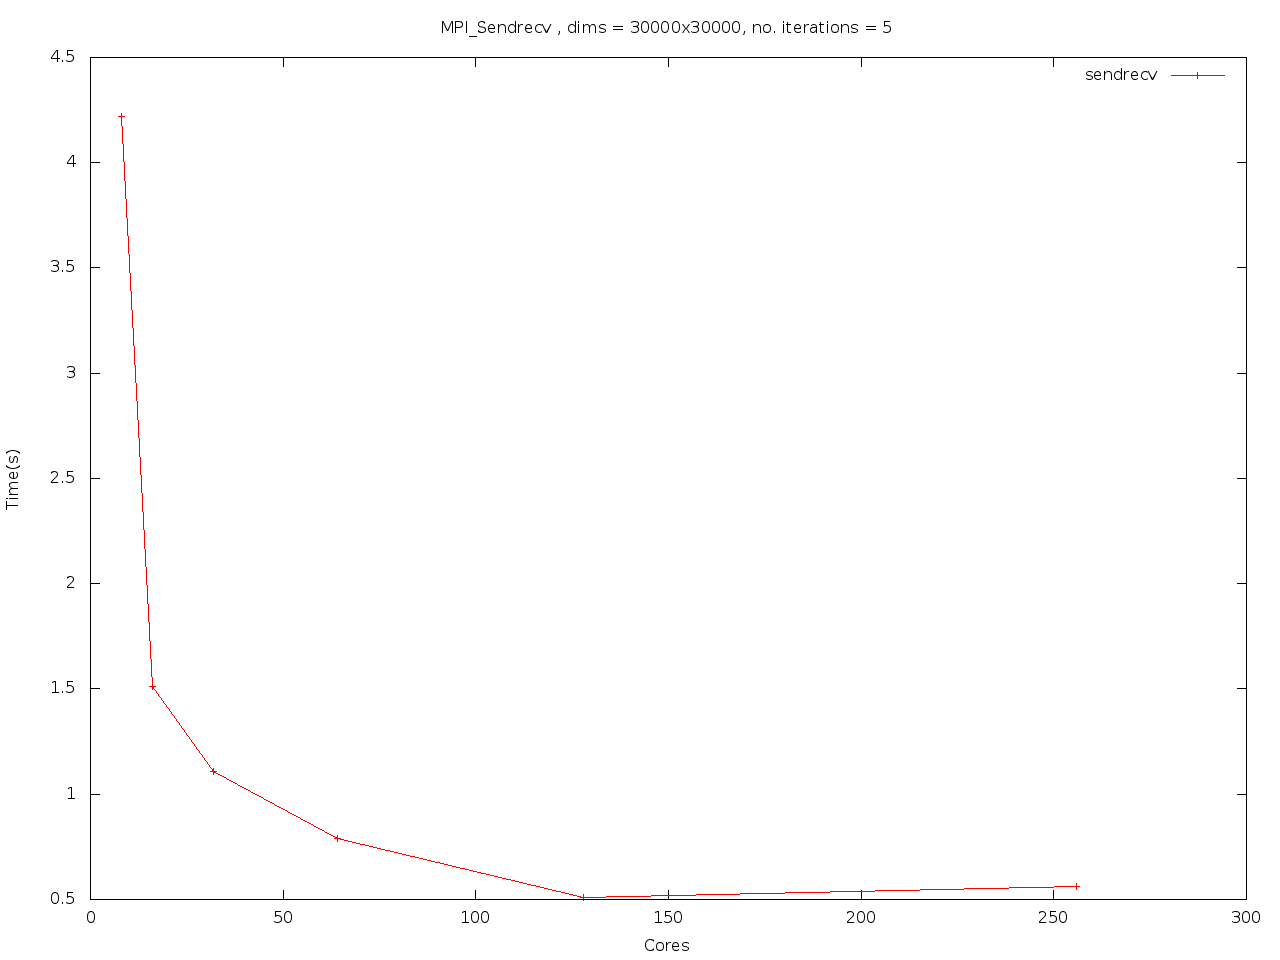
\includegraphics[width=0.7\textwidth]{srcxt.png}
\end{center}

As one can see from the graph, the MPI\_Sendrecv implementation behaves quite nicely with a rising number of cores. The curve looks similar to
the 1/n curve, but the time doesnt exactly halve with a doubled number of cores.

\subsection{Non-Blocking exchange}
The non blocking algorithm works in the same way as the sendrecv implementation, with the only difference that it uses the non-blocking $MPI\_Isend$
$MPI\_Irecv$ for the exchange. We also have to maintain a list of requests for each processor so that we can call MPI\_Waitall.
\begin{lstlisting}[label=some-code, caption=Non-blocking MPI left call + MPI\_Waitall]
      
MPI_Isend (&((*sub_matrix)[1]), 1, col, tmp_rank, 
    1, MPI_COMM_WORLD, &requests[reqs]);
MPI_Irecv (*sub_matrix, 1, col, tmp_rank, 
    3, MPI_COMM_WORLD, &requests[reqs]);

MPI_Waitall(reqs,requests,statuses);

\end{lstlisting}

\begin{center}
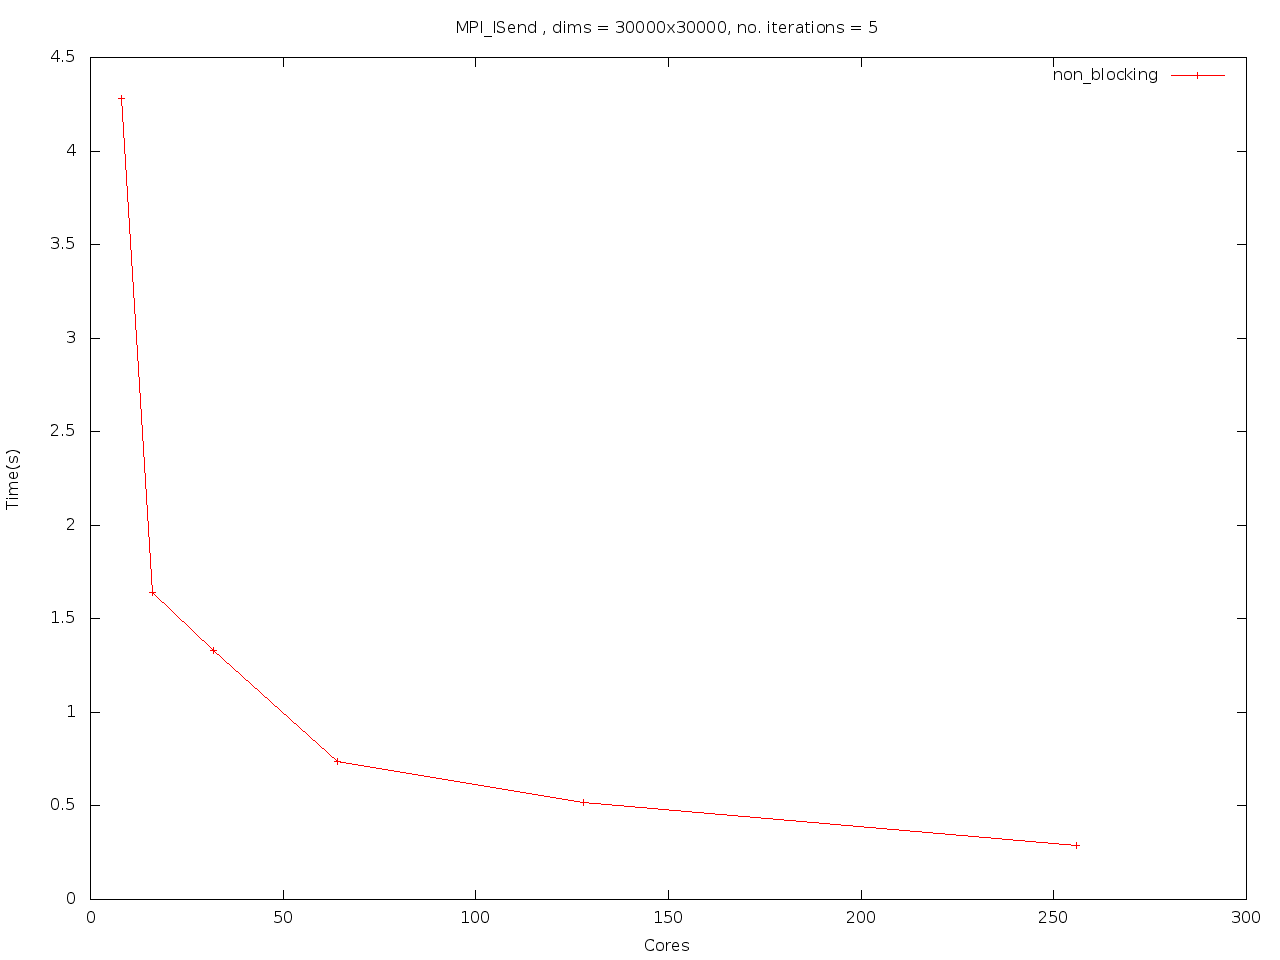
\includegraphics[width=0.7\textwidth]{nbcxt.png}
\end{center}

With respect to the dependency of the time to the number of cores, the curve here also behaves similarly to the one in the sendrecv implementation.

\subsection{MPI\_Put and MPI\_Get exchange}
Although it was not required, we also implemented a one-sided version of the exchange using MPI\_Get, to test how it would affect the performance 
compared to MPI\_Put. Both programs have to maintain a window for each processor, containing memory for the 4 boundaries of the node. In the case
MPI\_Put, after each put epoch (happening once per iteration) each process needs to copy the new values in the window to its own boundaries. On the
other hand, in the MPI\_Get version after each iteration each process must copy its new updated edges (but not boundaries) to the window. After that
every process gets their new boundaries from the windows of their respective neighours.
\begin{lstlisting}[label=some-code, caption=Left MPI\_Put vs left MPI\_Get call]
      
MPI_Put(&((*sub_matrix)[1]), 1, col, neigh_ranks[get_num], 
    2*SUB_COL + SUB_ROW, SUB_ROW, MPI_DOUBLE, win);

MPI_Get(*sub_matrix, 1, col, neigh_ranks[get_num], 
    2*SUB_COL + SUB_ROW, SUB_ROW, MPI_DOUBLE, win);

\end{lstlisting}

\begin{center}
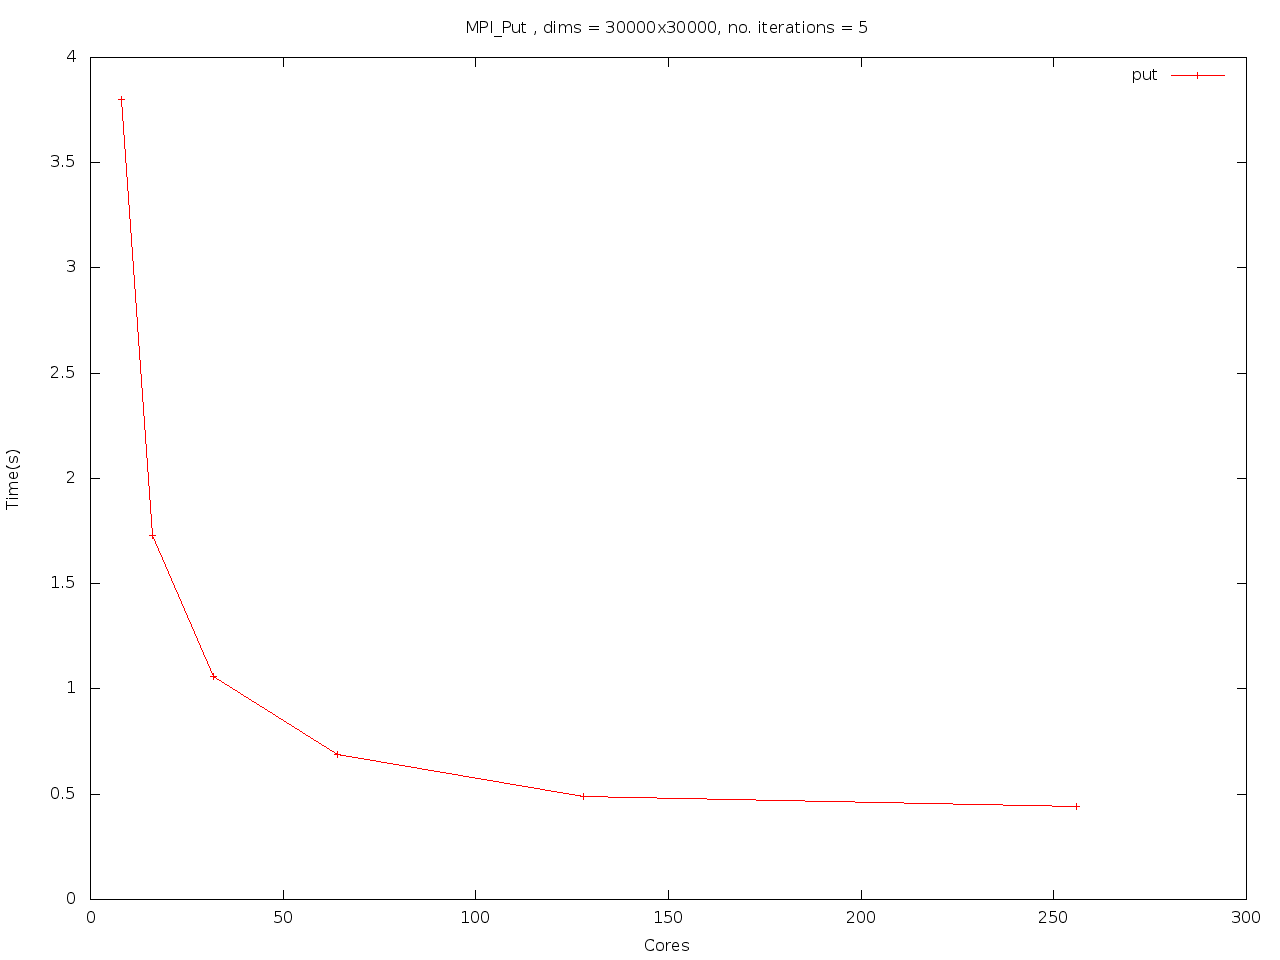
\includegraphics[width=0.7\textwidth]{putcxt.png}
\end{center}
\begin{center}
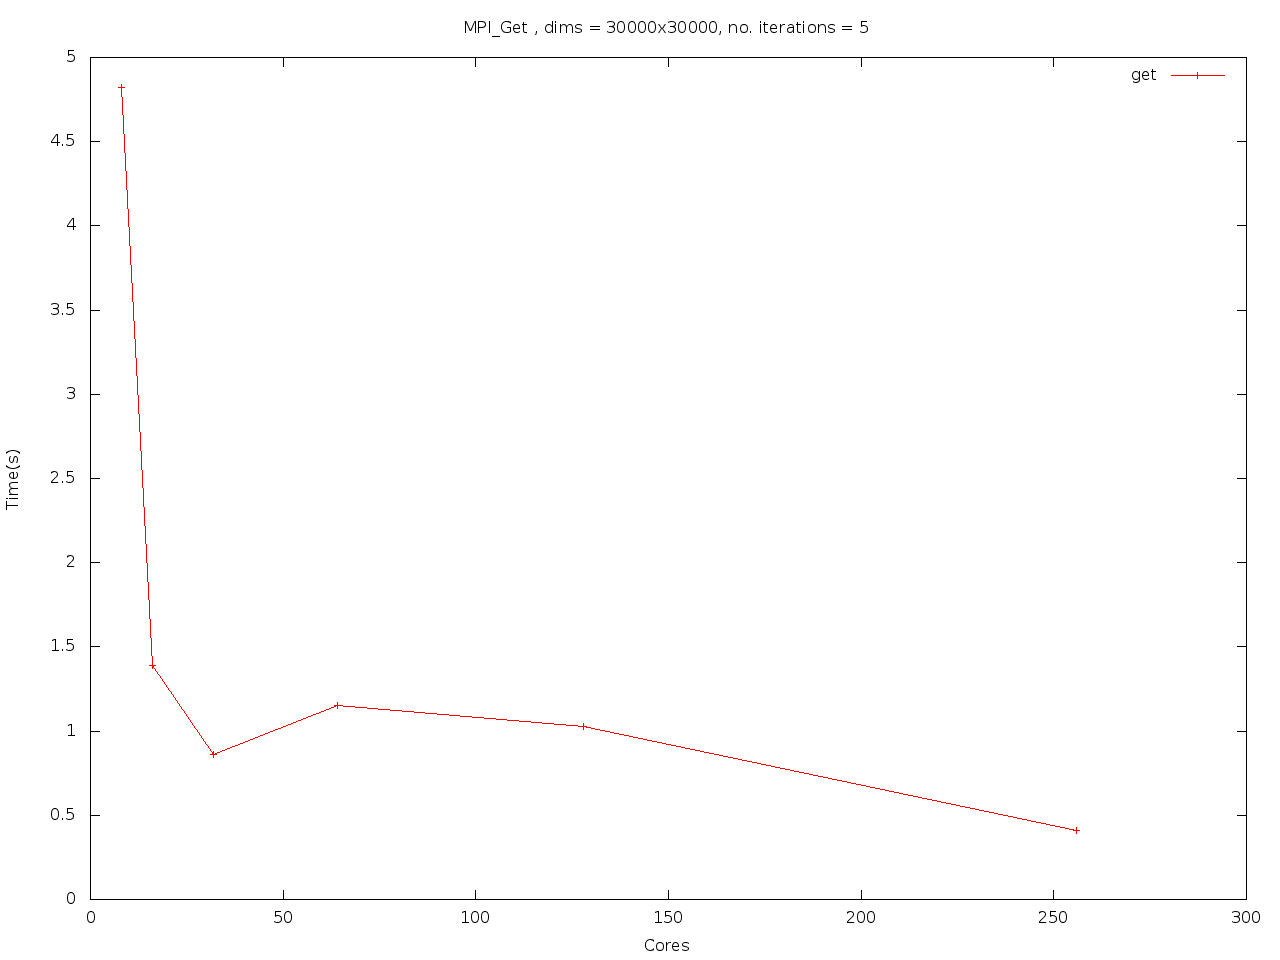
\includegraphics[width=0.7\textwidth]{getcxt.png}
\end{center}

As seen from the graphs, the $Time x Cores$ curve from the get and put implementations behave roughly the same as the other MPI implementations.
The slight rise in the MPI\_Get curve was likely caused by temporarily increased traffic at the jupiter server.
\subsection{MPI conclusion} 
Even though by using MPI we achieved by far the best $Cores x Time$ curves, the results still didn't exactly fit our hypothesis that there is an implementation that
lets the speedup increase linearly to the number of cores. But for 8, 16, 32 cores in our largest MPI test instances we achieved exactly this, so maybe this approach
comes as close as possible to achieving our goal.

\section{Correctness/testing} To test for correctness we used our special testing environment and script. For this purpose we created the testing folder which contains
the two test scripts test.py and test.sh, and the objectfiles of all out parallel programs stored in the respective folders. The test.py script simply tests compares the output of
any parallel algorithm to the output of the sequential row algorithm started with the same arguments. The test.sh scripts simply calls the test.py script for many different instances of the
parallel programs. The two resulting output files are compared using diff. If this function returns nothing, then both files are completely the same. Otherwise the test is declared as failed. 
I would like to believe that we also handled many of the extreme cases that can happen, although there are not so many extreme cases as far as stencil computation is concerned. The full list of
our test cases can be seen it he above mentioned test.sh (stencil/testing/test.sh)\\
Another interesting way to test our parallel stencil programs for correctness is to initialize the whole matrix (if the vectors are embedded in the array as in our implementation), starting from null
and incrementing for every cell. The result is a matrix that will never change, no matter how many times it is updated by our stencil program. The reason for this is that each cell is exactly the average
of all its neighbours (the one left and right are have a value of -1 and +1, and the ones up and down have a value of -(cols+2) and +(cols+2)). That is why we added the -t option in every program. With this option the
matrix is initialized as said above, and will should change after any number of updates if the implementation is correct.

\section{Experimental setup/Benchmarks}
Generally we feel that our MPI benchmarks on the jupiter server were a lot more successful than our openmp and cilk benchmarks at the saturn server. The reason for this is the very large traffic on the saturn server during
the running of our benchmarks. With on jupiter, we largely managed to avoid this traffic by mainly using the last nodes (18,17,16...), because most of the other participants simply started their benchmarks from the first nodes (because of the default login in 0), where the
traffic was the largest. We sadly had no way of avoiding the traffic on the saturn server, and this is why we feel that our benchmarks don't properly display the actual speedup achieved with our parallel implementations. For this reason, we also made more limited benchmarks locally,
that should more accurately display the real speedup of our parallel programs.\\
\subsection{Benchmarking setup}
For the benchmarks on both saturn and jupiter we used we used a similar approach. We divided our benchmarks in stages, with each stage increasing the size of the datasets and the set of cores used, 
but decreasing the number of iterations and the number of repetitions. This way, the execution time doesn't increase drastically with the increasing data sizes, so our benchmarks finish in a shorter time, 
sadly at the cost of some accuracy in the measurements. We did not benchmark the extreme cases, as these appear rarely in the real world, but focused our benchmarks on square or rectangular matrices, where the one side
is maximally 3-4 time bigger than the other. We used two sets of 8 elements for our columns and rows and separated them into two subsets of two values for each stage. We then combined each element of one subset with each element of the
other subset to get 4 different dimensions for every stage. In the MPI benchmarks we used 100 iterations and 10 repetitions for the 1st stage, 50 and 7 for the second, 10 and 5 for the third and 5 and 2 for the last. We built the average, 
median and minimum for each set of repetitions, and manually took the value we thought fitted the set of observed times the best. Our approach for the cilk and omp benchmarks was similar. We took the same sizes as in the MPI benchmarks, and used
10000, 1000, 100 and 10 iterations for the 1st, 2nd, 3rd and 4th stage respectively and took 20, 10, 5 and 5 repetitions for the respective stages. It also important to note that we decided to predominately take the minimum, not the average for our
plots, because of the traffic we encountered on the saturn server.
We also ran slightly limited benchmarks for cilk and omp on our local computer, to more accurately 
display the speedups with a smaller number of processors and smaller datasets. We also benchmarked some of the algorithms that were inherently slower, (columnwise, diagonal iteration, space efficient algorithm) only for smaller instances, because
benchmarks would become unreasonably long for the large instances.
\begin{lstlisting}[label=some-code, caption=The two sets of sizes used for the rows and columns]
rows = [32, 100, 400, 1000, 2800, 6400, 10000, 30000]
cols = [64, 100, 600, 1000, 5200, 7600, 10000, 30000]
\end{lstlisting}

\subsection{Benchmarking results}
Now we present the results of the MPI benchmarking as plots and just explain these briefly, because we feel that the plots can express more than what we could summarize in a few sentences.
\subsubsection {MPI}
\begin{center}
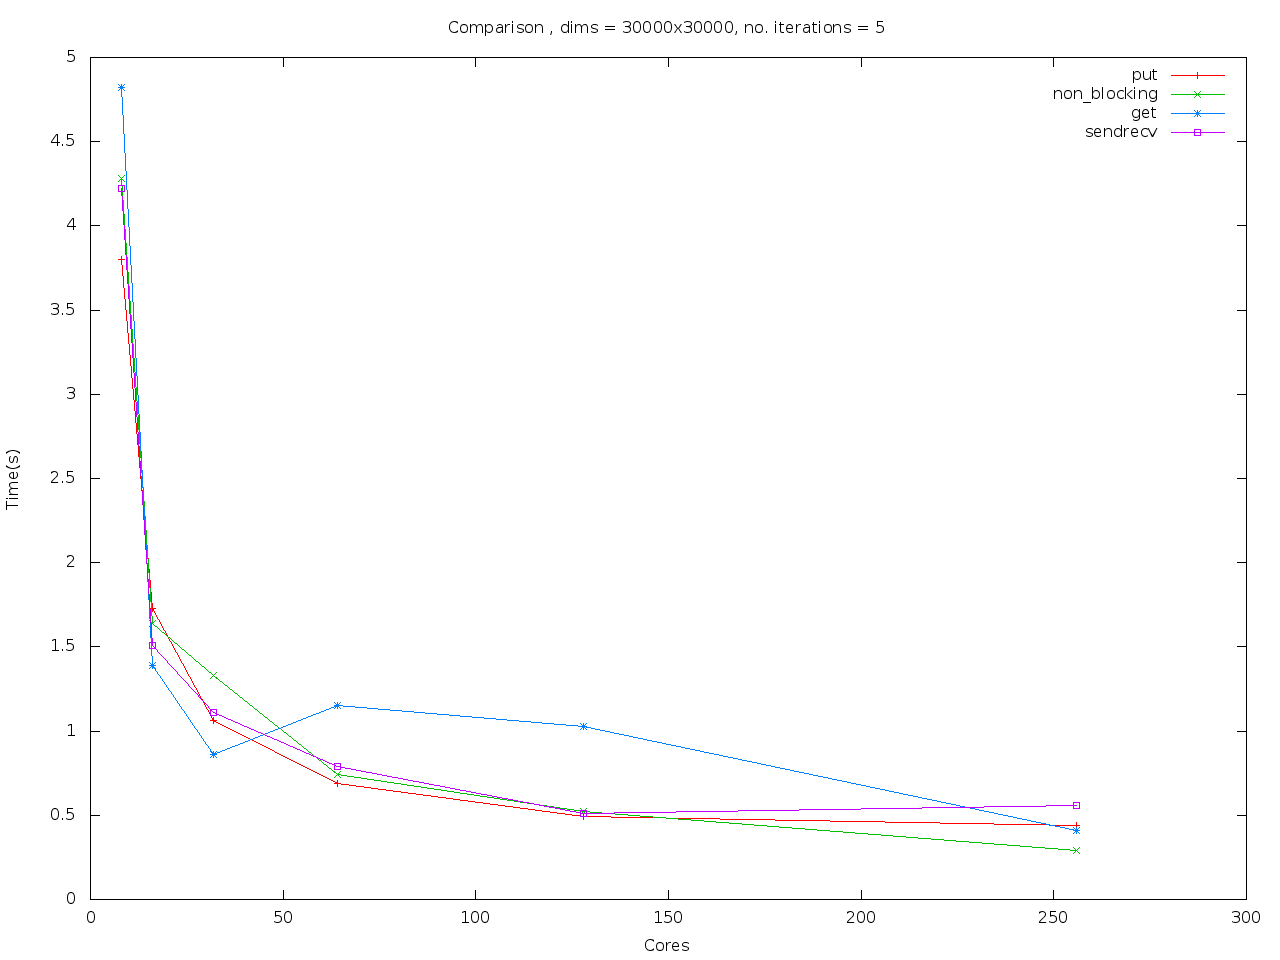
\includegraphics[width=0.7\textwidth]{cmpcxt.png}
\end{center}
This graph compares all 4 MPI implementations w.r.t. the dependency of times from the number of cores used for the largest dataset(30000x30000).
On this graph we can see what already displayed in the MPI section, namely that the times reduces quite nicely by increasing the number of cores.
\begin{center}
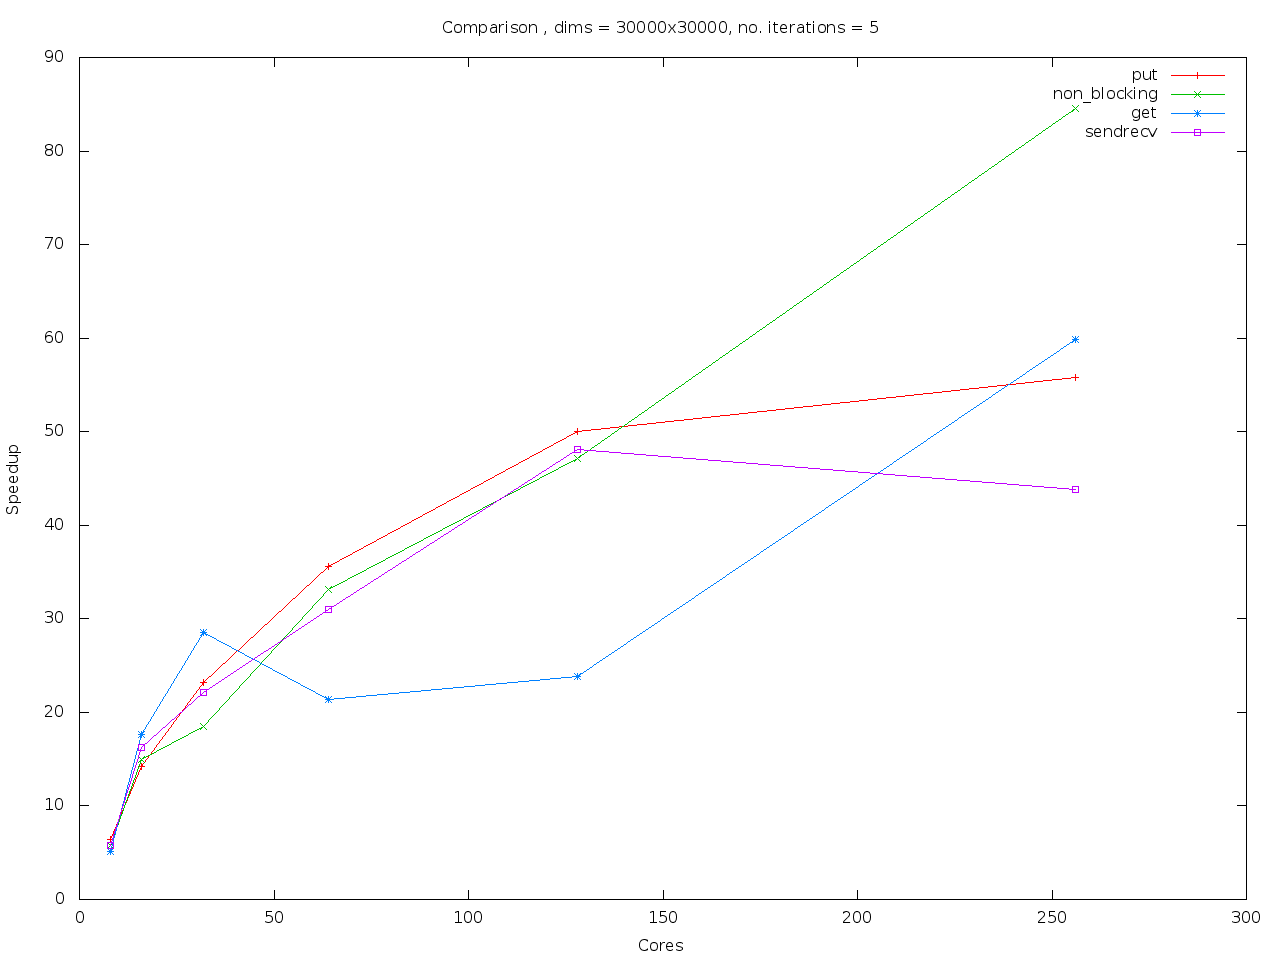
\includegraphics[width=0.7\textwidth]{cmpsxc.png}
\end{center}
This graph is closely connected to the previous graph, as it displays the dependency between the speedup and the number of cores for the largest instance(the speedup is calculated by (seqtime/partime)).
The maximum speedup was achieved with the non-blocking MPI implementation, where the observed time using 256 cores was 84.6 times faster than the sequential time for the same instance. The other versions of the
program also achieved relatively large speedups, being consistently at least 40 times faster than the sequential algorithm when using 256 cores.
\begin{center}
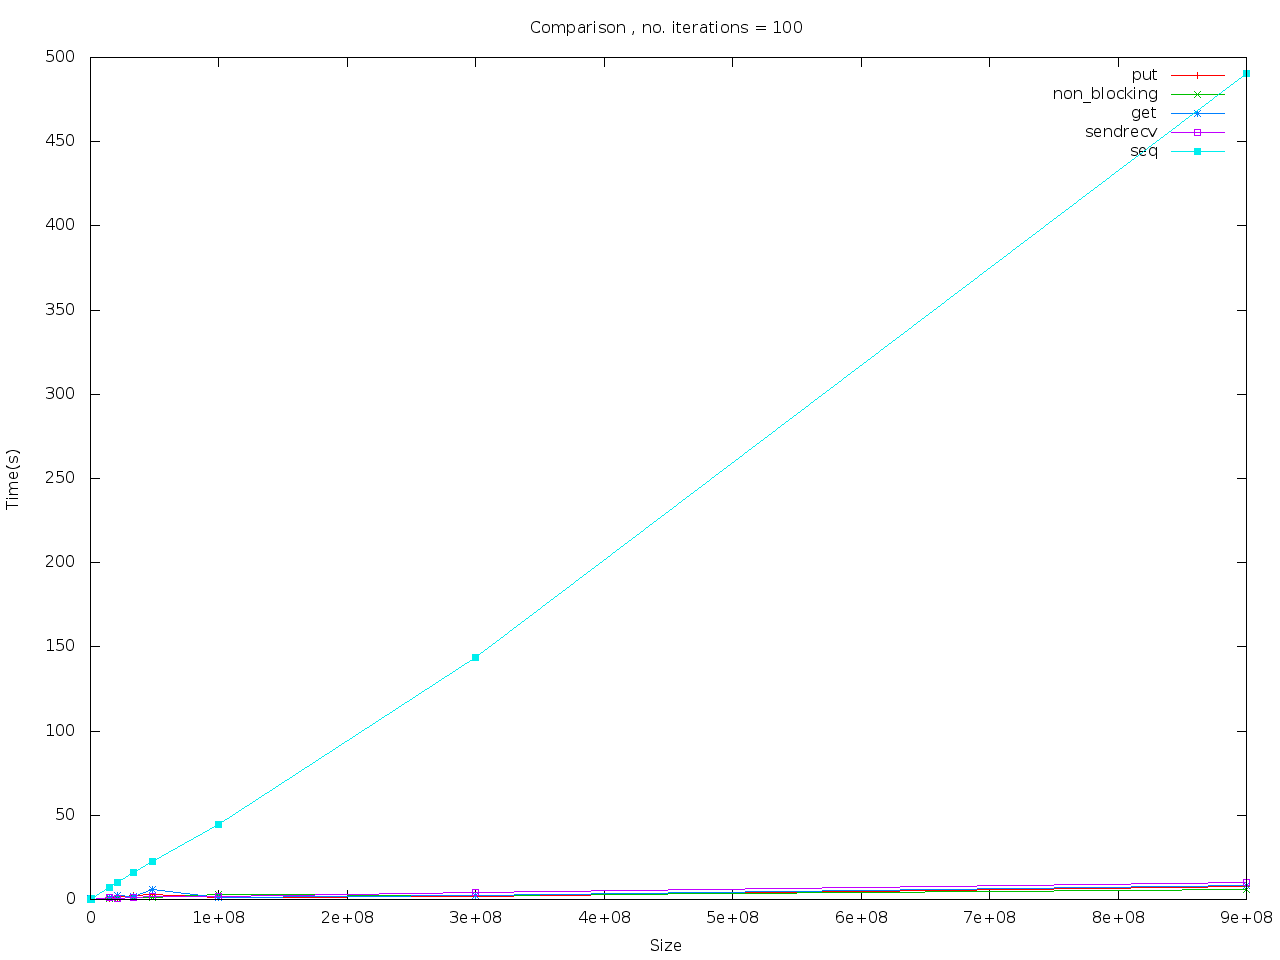
\includegraphics[width=0.7\textwidth]{cmpsxt.png}
\end{center}
This graph shows how different dataset sizes affect the measured time for each MPI algorithm and the sequential algorithm. For the parallel algorithms, for each size, we took the average time measured with the number of cores
that produced the best results for this instance. As you can see, at the large instances the MPI implementation largely outperform the sequential implementation, namely so much, that we can barely tell the difference between the
MPI implementation plots.
\begin{center}
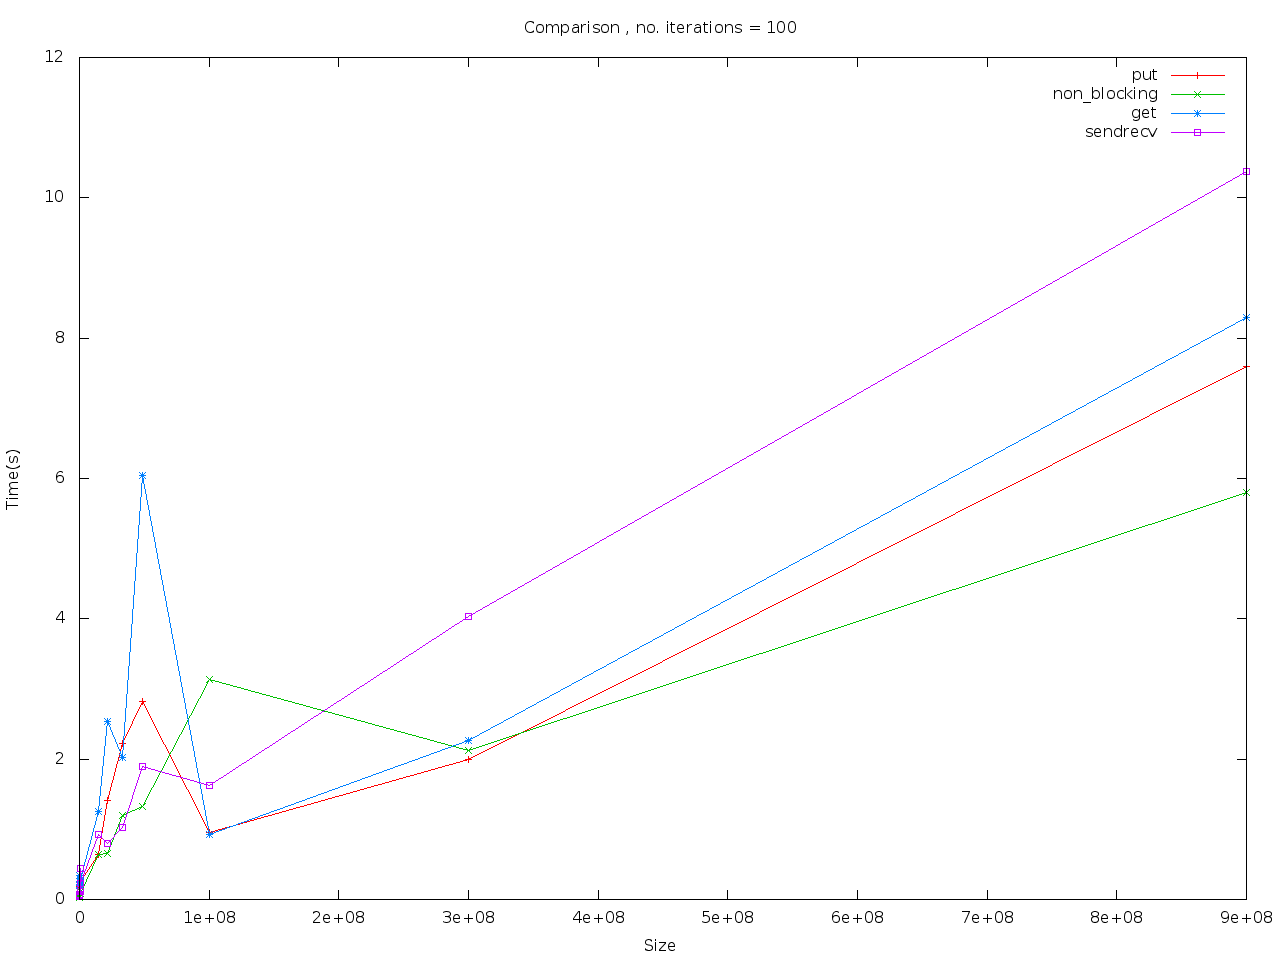
\includegraphics[width=0.7\textwidth]{cmpsxtnoseq.png}
\end{center}
The final graph displays the same information as the previous graph, only this time excluding the sequential implementation plot.
As we can see, the all the algorithms tend to perform badly for small instances, because the communication costs exceed the slight gain
achieved through parallelization, but at the larger instances, the use of a lot of cores starts bringing significant speedups. We can see
that the time still grows linearly w.r.t. the dataset size(on the larger instances), but the factor is simply a lot smaller than the factor seen
at the sequential implementation plot.


\subsection {CILK \& OMP \& Sequential Space-Opitmized Algorithm }
\begin{center}
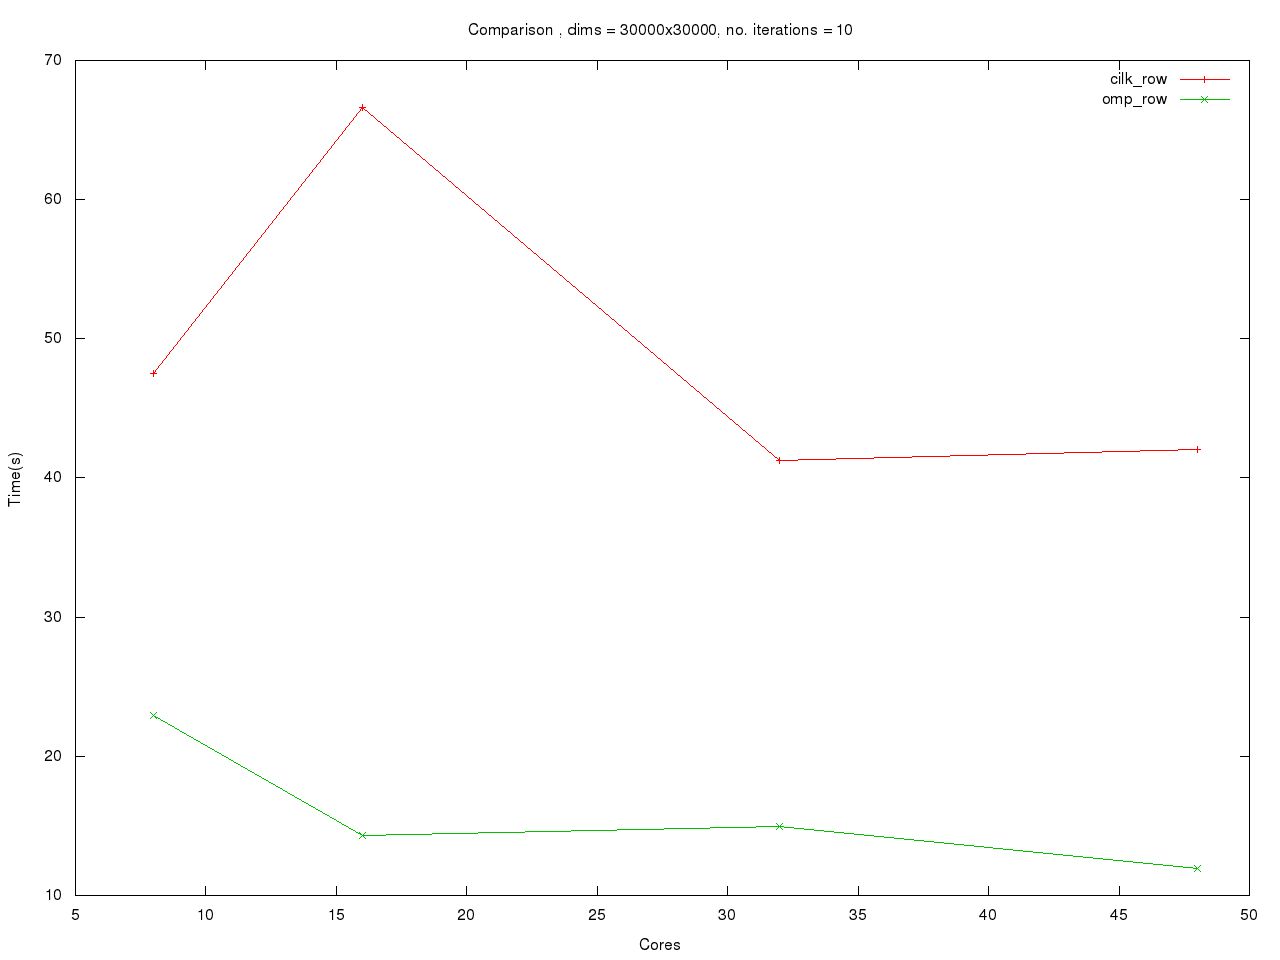
\includegraphics[width=0.7\textwidth]{compcxtompcilk.png}
\end{center}
This graphic allows us to see the what the change in time more (or less cores) cause in different environments, but with the same number of iterations and dimensions.\\
In OMP we see a tremendous increase in performance as the number of cores increases. This increase in performance has it's peak at 16 cores, then the overhead of the framework trying to parallelize the data weighs it down. \\
Cilk on the other hand doesn't seem to take much advantage of the number of cores, but also stays stable in comparision, it starts to slow down at a later point and slower rate than OMP, because (as we can see the in the next chart) OMP has a much better speedup rate in general than Cilk.


\begin{center}
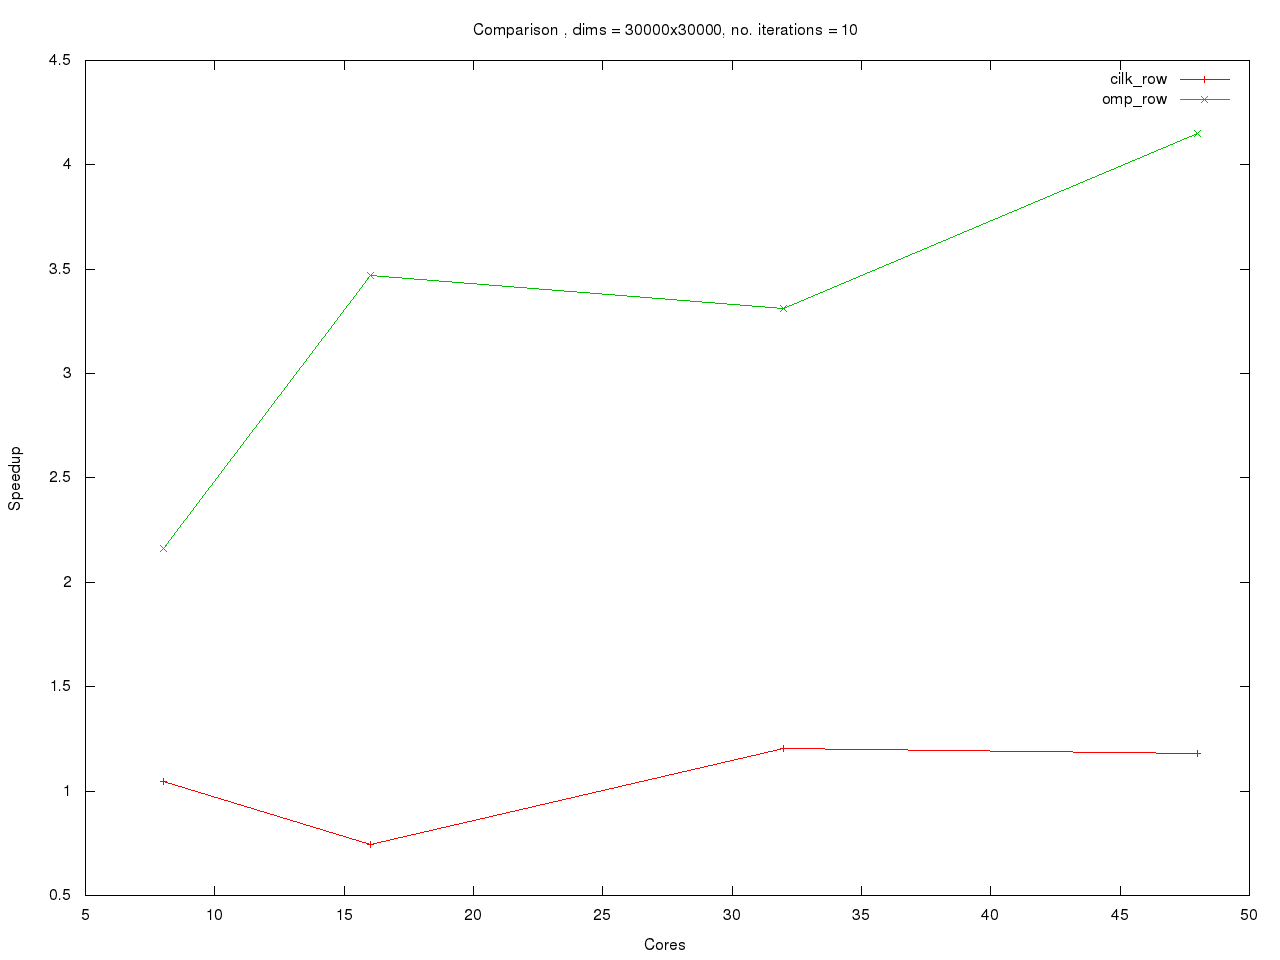
\includegraphics[width=0.7\textwidth]{compsxcompcilompcilkseqk.png}
\end{center}
This chart shows the actual difference in speedup of both frameworks in processing a certain amount of data. As previously mentioned, the speedup of OMP is much greater, almost linear but with a slowdown factor.\\
Cilk doesn't have a linear speedup at all and is being rather constant over a greater amount of cores.\\
The maximal amount of speedup caused by OMP is approximately $\approx4.2x$, caused by 48 cores while the maximal speedup of Cilk is just $\approx1.3x$, also caused by 48 cores, or alternatively 32.
\begin{center}


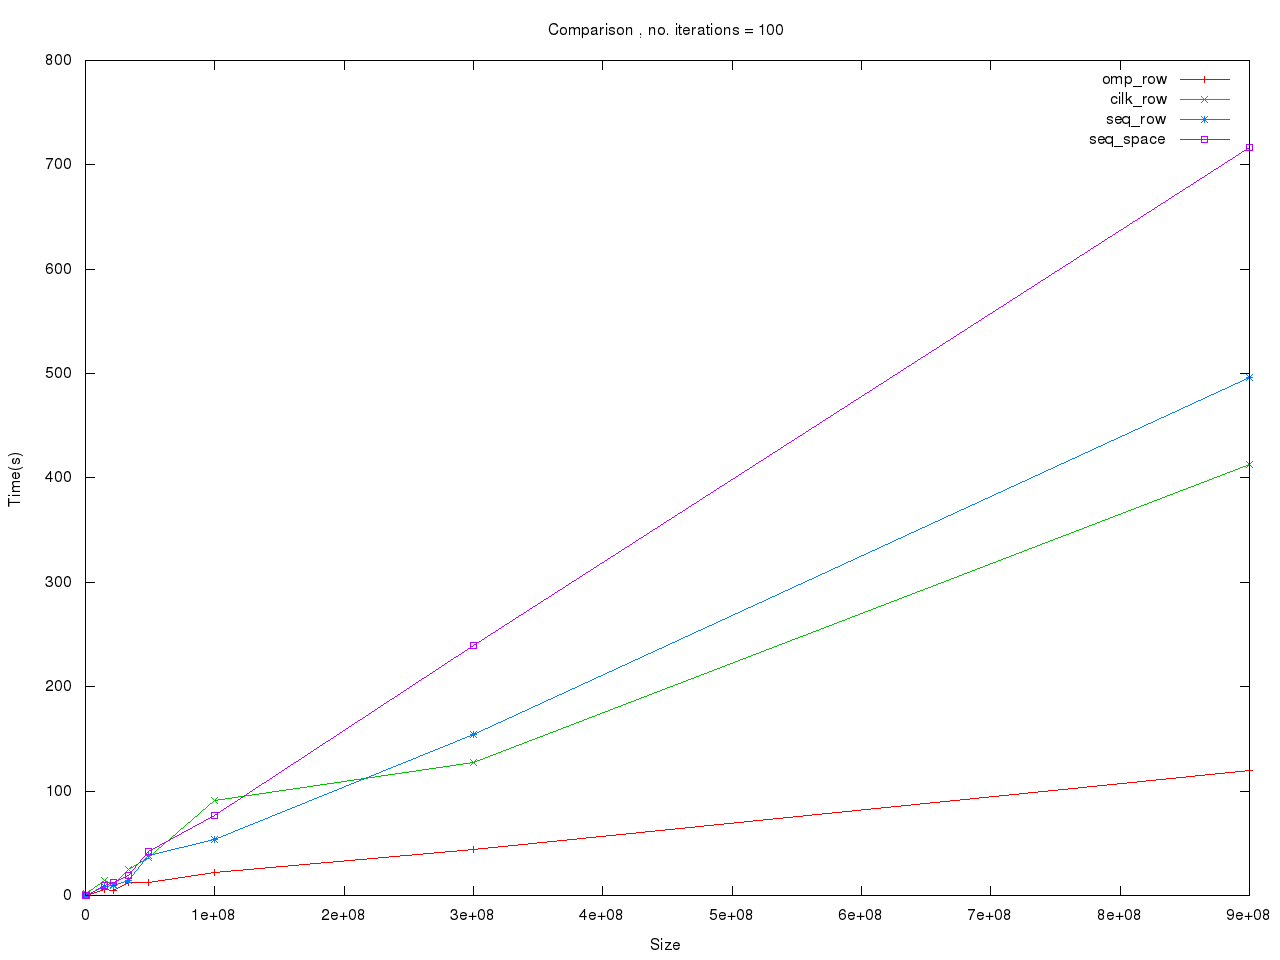
\includegraphics[width=0.7\textwidth]{compsxtompcilkseq.png}
\end{center}
We can see that in this graph the relation of the size of the matrix which has to be computed by our stencil computation and the time that is needed to do such thing.\\
While the sequential memory-optimized version (called seq\_space in the graph) takes more time but still scales well. \\
The 'normal' sequential version scales approximately linearily, Cilk has a overhead which reduces the scaling effect on small sample sizes, but it still enables the time to be reduced. OMP scales best of all the versions, a ratio of time/size of $\approx5$.


\section{Conclusion}
First we cannot draw any definite conclusions for the shared-memory implementations on the saturn server because it was overloaded by all other students running their benchmarks, which negatively impacted the performance of our parallel programs. \\
Still we can conclude that OMP was more suited to out stencil-update problem than Cilk because OMP is data-parallel oriented whereas Cilk is talk-parallel oriented which isn't suited to our problem.\\
This can also be seen on the benchmarks we did. \\
Our conclusion regarding the shared-memory parallel frameworks like Cilk and OpenMP is that a good speedup can be achieved up to 16 cores for bigger datasets, but dividing the computation to even more cores will either not change the performance or impact it negatively, because of the synchronization overhead.\\ 
With the MPI framework on the other hand, manage to achieve a much better speedup as compared to the shared memory frameworks and the speedup kept increasing even when using 256 cores. The benchmarking of the Jupiter distributed system was also easier because we could avoid the trafic created by the other students by executing the benchmarks mostly on the less used nodes of the system. With MPI we manage to achieve out maximal speedup of 84.6 times compare to the fastest sequential algorithm we had.\\
The speedup however does not include the overhead created when scattering and gathering the matrix. The above mentioned overhead can take most of the computation time when executing the program on large datasets with a small number of iterations so we recommend using the distributed system when the stencil computation requires a large number of iterations.
For a small number of iterations we would choose to use the OMP-implementation of our 2d-stencil program. 






\end{document}
